\chapter{게이지 장, 상호작용 척도 및 하전 약전류}

양자전기역학과 양자색역학은 실험실에서 보면 매우 달라 보이지만, 둘 다 게이지 이론이다. 사실 표준모형의 거의 모든 상호작용은 이런 방식으로 구성된다. \emph{게이지}라는 말에는 국소 대칭과 관련된 더 깊은 의미가 있지만, 그 수학적 틀은 뒤로 미뤄도 된다. 지금은 최소한의 물리적 설명이면 충분하다. 게이지 이론에는 맥스웰 이론과 비슷한 장, 보존되는 원천, 대칭 변환, 게이지 보손, 그리고 그 보손을 방출하고 흡수하는 규칙이 들어 있다.

\section{원형이 되는 맥스웰 이론}

\subsection{장과 퍼텐셜}

전자기장은 성분이 여섯 개다. 전기장 성분이 셋, 자기장 성분이 셋이다. 이와 같은 정보를 중복성을 허용하는 사차원 벡터 퍼텐셜로 나타낼 수도 있다.
\begin{equation}
A_\mu=(A_0,\boldsymbol A),
\end{equation} 여기서 \(A_0\)는 정전기 퍼텐셜이고 \(\boldsymbol A\)는 공간 벡터 퍼텐셜이다. 정전기적 한계에서는 공간 기울기로부터 전기장을 구한다.
\begin{equation}
\boldsymbol E=-\boldsymbol\nabla A_0,
\qquad
\boldsymbol F=q\boldsymbol E,
\end{equation} 한편 자기장은 다음과 같다.
\begin{equation}
\boldsymbol B=\boldsymbol\nabla\times\boldsymbol A.
\end{equation} 첫 번째 식의 부호는 퍼텐셜의 표준적인 정의에 따라 달라진다. 칠판에서 다룬 핵심은 장이 퍼텐셜의 미분으로 주어진다는 점이다.
\editorialnote{시간에 따라 변하는 장의 완전한 관계식은 다음과 같다.
\(\boldsymbol E=-\boldsymbol\nabla A_0-\partial_t\boldsymbol A\) 여기서는 의도적으로 더 단순한 정전기적 수준에서 설명한다.}

\begin{figure}[htbp]\centering
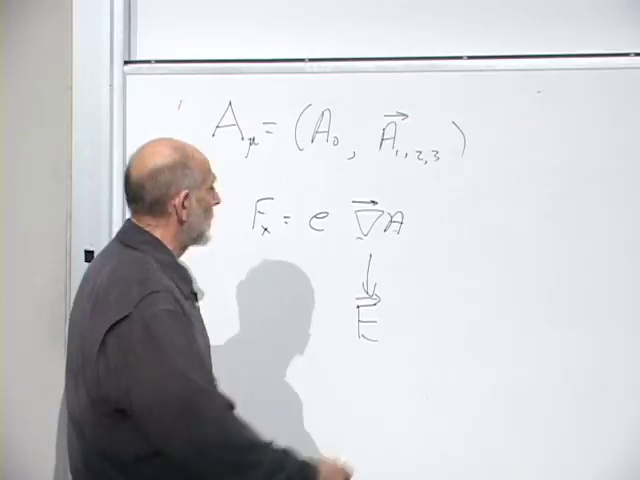
\includegraphics[width=0.62\textwidth]{lecture_05_figure_02.png}\caption{전자기 사차원 퍼텐셜과 장에 대한 미분 관계.}\lectureframe{00:03:33}\end{figure}

따라서 전기역학은 서로 동등한 두 가지 방식으로 기술할 수 있다. 하나는 \(\boldsymbol E\)와 \(\boldsymbol B\)를 사용하는 방식이고, 다른 하나는 \(A_\mu\)를 사용하는 방식이다. 후자에 표시된 성분은 네 개뿐인데, 서로 다른 퍼텐셜이 동일한 물리적 장을 나타낼 수 있기 때문이다. 이 중복성이 게이지라는 말의 배경을 처음으로 보여 주지만, 아직 형식적으로 사용하지는 않겠다.

\subsection{파동과 편광}

맥스웰 방정식은 파동을 허용한다. 단위 벡터 \(\hat{\boldsymbol k}\) 방향으로 진행하는 평면파를 생각해 보자. 모든 지점에서 전기장과 자기장은 횡방향이다.
\begin{equation}
\boldsymbol E\cdot\hat{\boldsymbol k}=0,
\qquad
\boldsymbol B\cdot\hat{\boldsymbol k}=0,
\qquad
\boldsymbol E\cdot\boldsymbol B=0.
\end{equation} \(c=1\)인 단위계에서는 두 장의 크기가 같다.
\begin{equation}
|\boldsymbol E|=|\boldsymbol B|.
\end{equation} 선편광파에서는 \(\boldsymbol E\)의 방향이 편광을 지정한다. 파동의 전체 무늬는 빛의 속도로 전파된다.

양자화는 서술 방식을 바꾸지만 편광 구조는 바꾸지 않는다. 전자기파의 양자는 광자다. 광자를 점으로 그리면 필연적으로 오해를 부르지만, 그 점이 편광을 나타내는 작은 횡방향 화살표를 지닌다고 상상하면 유용하다. 사분파장판이나 다른 광학 소자는 그 편광을 회전시킬 수 있다. 정적인 쿨롱 장도 아주 거칠게나마 광자의 반복적인 방출과 흡수에서 생긴다고 그려 볼 수 있다.

\subsection{원천, 플럭스 및 보존}

전자기파는 빈 공간에서도 전파되지만, 장에는 전하와 전류라는 원천도 있다. 양전하를 띤 점전하는 \(1/r^2\)에 비례하는 바깥쪽 방사형 전기장을 만든다. 전하를 둘러싼 구면을 통과하는 장선의 수는 구면의 반지름과 무관하다. 수식으로 쓰면 다음과 같다.
\begin{equation}
\oint_{S^2}\boldsymbol E\cdot d\boldsymbol S
=\frac{Q_{\mathrm{enc}}}{\epsilon_0},
\label{eq:l5-gauss}
\end{equation} SI 단위계에서의 식이다.

이는 장을 계산하는 편리한 방법에 그치지 않는다. 전기장선은 전하에서만 끝날 수 있다. 고립된 전하 하나가 그저 사라진다면, 인과율을 위반하면서 그 장이 모든 곳에서 동시에 사라져야 한다. 그렇지 않으면 장선이 빈 공간에서 끝나는, 장이 사라진 영역의 경계가 바깥으로 전파되어야 한다. 둘 다 허용되지 않는다. 따라서 선속의 기하학적 구조는 전하 보존을 자연스럽게 만든다. 전하는 움직일 수 있고 서로 반대인 전하는 소멸할 수 있지만, 보상하는 전류 없이 순전하가 국소적으로 사라질 수는 없다.

이에 대응하는 국소적 진술은 연속 방정식이다.
\begin{equation}
\partial_t\rho+\boldsymbol\nabla\cdot\boldsymbol J=0.
\label{eq:l5-continuity}
\end{equation}
\editorialnote{~\eqref{eq:l5-continuity} 방정식은 강의에서 말로 전개한 인과적 선속 논증을 표준적인 국소 수학 형식으로 나타낸 것이다.}

\subsection{게이지 이론의 실용적 정의}

이제 작동상의 전형을 서술할 수 있다. 게이지 이론에는 다음이 있다.
\begin{itemize}\item 전기장과 유사한 장 및 자기장과 유사한 장;
\item 상호작용이 충분히 약할 때 빛의 파동과 비슷한 파동;
\item 전하와 유사한 원천;
\item 선속과 그 원천을 연결하는 가우스 법칙;
\item 보존 법칙과 이에 대응하는 대칭;
\item 게이지 보손이라 부르는 장의 양자;
\item 방출과 흡수를 제어하는 결합 상수.
\end{itemize}
원천이 반드시 전하일 필요는 없다. 의도적으로 비현실적인 예로 바리온 수를 게이지 대칭으로 만든다고 상상해 보자. 양성자와 중성자는 모두 바리온 수 \(+1\)를 가지므로 새로운 쿨롱 유사 힘으로 서로 밀어내고, 양성자와 반양성자는 서로 끌어당길 것이다. 이런 이론은 수학적으로 상상할 수 있지만, 자연에는 바리온 수와 결합하는 장거리 게이지 장이 관측되지 않는다. 보존 법칙이 있다고 해서 게이지 힘까지 반드시 존재하는 것은 아니다.

전하에는 실제로 대칭이 따른다. 전하를 띤 물질장에 대해,
\begin{equation}
\psi(x)\longmapsto e^{i\theta}\psi(x).
\label{eq:l5-u1}
\end{equation}
위상 대칭과 전하 보존은 같은 구조의 양면이다. 나중에 \(\theta\)를 시공간에 따라 달라지게 해 보면 퍼텐셜 \(A_\mu\)가 왜 필요한지 알 수 있다. 여기서는 전역 변환만으로도 보존 전하를 확인하기에 충분하다.

\section{비아벨 예로서의 양자색역학}

\subsection{삼중항, 반삼중항 및 글루온 행렬}

양자색역학에서 쿼크장은 색 지표 \(i\in\{r,g,b\}\)를 가지며 \(SU(3)\)의 기본 표현으로 변환한다.
\begin{equation}
q'_i=U_{ij}q_j,
\qquad
U^\dagger U=\boldsymbol 1,
\qquad
\det U=1.
\label{eq:l5-q-transform}
\end{equation} 이는 삼차원 복소 색 공간에서의 회전이지, 통상적인 위치 공간의 회전이 아니다. 삼차원 표현은 정의 표현이라고도 부른다.

반입자 장은 복소켤레 변수로 나타낸다. 식~\eqref{eq:l5-q-transform}의 복소켤레를 취하면 다음과 같다.
\begin{equation}
q_i^{\prime *}=U_{ij}^*q_j^*.
\label{eq:l5-antiquark-transform}
\end{equation} 따라서 쿼크는 \(\boldsymbol 3\)로 변환하고, 반쿼크는 \(\bar{\boldsymbol 3}\)로 변환한다.

\begin{figure}[htbp]\centering
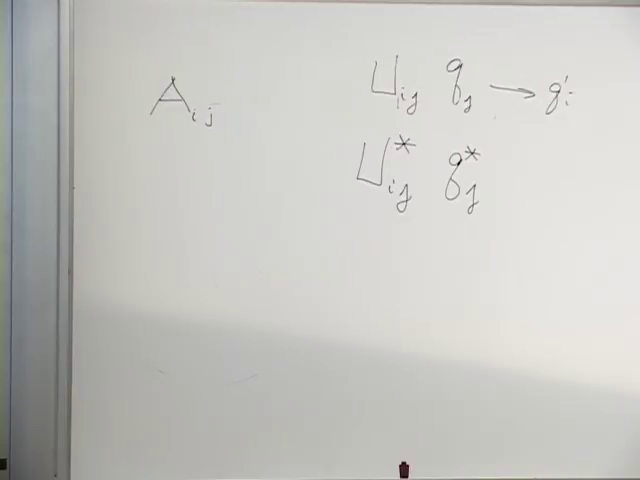
\includegraphics[width=0.62\textwidth]{lecture_05_figure_03.png}\caption{기본 표현의 변환과 그 복소켤레인 반삼중항 표현의 변환.}\lectureframe{00:18:47}\end{figure}

\begin{classroomqa}\audiencequestion{\(U\) 행렬은 몇 개입니까-- 일곱 개, 여덟 개, 아홉 개입니까?
\lecturetimestamp{00:19:37}}\lecturerresponse{군의 원소 \(U\)는 무한히 많습니다. 세는 대상은 독립 생성자의 유한한 개수이며, \(SU(3)\)의 경우 여덟 개입니다. 일반적인 \(3\times3\) 행렬에는 행렬 성분 자리가 아홉 개 있지만, 특수 유니터리 조건 때문에 연속적인 방향은 여덟 개만 남습니다.}\end{classroomqa}

글루온 장은 흔적이 없는 행렬 \(A_{ij}\)로 쓸 수 있다. 한 지표는 쿼크처럼, 다른 지표는 반쿼크처럼 변환하므로 색 구조는 다음과 같다.
\begin{equation}
\boldsymbol 3\otimes\bar{\boldsymbol 3}
=\boldsymbol 1\oplus\boldsymbol 8.
\end{equation} 양자색역학은 흔적이 없는 팔중항을 취하고,
\begin{equation}
A_{ii}=\operatorname{tr}A=0,
\end{equation} 단일항은 제외한다. 그래서 양자색역학에는 아홉 개가 아니라 글루온 여덟 개가 있다. 더 일반적으로 \(SU(N)\)에는
\begin{equation}
N^2-1
\end{equation}개의 생성자와 같은 수의 게이지 보손 장이 있다.

광자는 전기 \(U(1)\)에 대해 중성이다. 전자의 위상을 회전시켜도 광자가 다른 광자로 바뀌지는 않는다. 글루온은 다르다. 글루온은 색과 반색을 띠므로 수반 표현으로 변환한다. 예를 들어 빨강--반파랑 조합은 색 하나와 반색 하나를 포함하지만 색 단일항은 아니다.

\subsection{지표의 흐름과 자기 상호작용}

지표를 따라가면 상호작용 규칙을 읽을 수 있다. 개략적으로 색 \(i\)을 가진 쿼크는 색 \(j\)을 가진 쿼크로 바뀌면서 이에 대응하는 색 흐름을 지닌 글루온을 방출할 수 있다.
\begin{equation}
q_i\longrightarrow q_j+A_{ij}.
\label{eq:l5-quark-gluon-vertex}
\end{equation} \(i\)와 \(j\)의 정확한 위치는 화살표 관례에 따라 달라진다. 불변인 내용은 꼭짓점에 들어오는 모든 지표가 다른 선을 통해 이어져야 한다는 점이다. 색 지표가 사라지는 일은 없다.

이 규칙은 모든 \(SU(N)\) 게이지 이론에 적용된다. 기본 표현의 물질은 지표 하나를, 반기본 표현의 물질은 켤레 지표 하나를 가지며, 게이지 보손은 각각 하나씩 가진다. 물리적 명칭은 달라질 수 있지만 지표 구조는 그대로다.

글루온 자체가 색을 띠기 때문에 다른 글루온을 방출할 수 있다. \(A_{ij}\) 글루온은 중간 지표 \(k\)를 거쳐 개략적으로 다음과 같이 분열할 수 있다.
\begin{equation}
A_{ij}\longrightarrow A_{ik}+A_{kj}.
\label{eq:l5-three-gluon-index}
\end{equation} 이는 완전한 양--밀스 꼭짓점은 아니지만 색 흐름을 보여 준다. 통상적인 전기역학에서 광자에는 이와 비슷한 일이 일어나지 않는다. 따라서 글루온은 글루온에 힘을 가하며, 비아벨 장 동역학은 맥스웰의 선형 이론보다 훨씬 복잡하다.

정성적인 결과 가운데 하나는 가둠이다. 색 선속선은 끝날 수 없으며, 선속선 사이의 자기상호작용은 쿼크와 반쿼크를 잇는 관을 만든다. 이 관은 길이 단위당 거의 일정한 에너지를 지닌다.
\begin{equation}
V(R)\simeq \sigma R.
\end{equation} 따라서 양 끝을 더 멀리 당기면 색을 띤 입자를 자유롭게 풀어 주는 대신 에너지가 더 저장된다. 이것이 끈적한 접착제라는 그림이다. 장 자체가 색을 띤 구성 요소들이 자유 입자로 빠져나오지 못하게 한다.

\section{결합 상수와 강함 또는 약함의 의미}

\subsection{방출 진폭으로서의 전하}

게이지 이론에는 여전히 결합 상수가 필요하다. 양자전기역학에서 전자 전하 \(e\)는 전자--광자 꼭짓점에 해당하는 계수다. 이는 진폭이며, 확률은 진폭의 제곱이다. 작동상의 의미를 보려면 음극선관에서 빠른 전자를 갑자기 멈춘다고 생각해 보자. 광자를 복사할 확률은 \(e^2\)에 비례하며, 관례적인 인자들은 미세구조 상수에 포함된다.
\begin{equation}
\alpha=\frac{e^2}{4\pi\hbar c}
\simeq \frac{1}{137}.
\label{eq:l5-alpha}
\end{equation} 자연 단위계 \(\hbar=c=1\)에서는 결합이 무차원이다. 기본 입자의 방출 척도가 일 퍼센트 정도이므로 섭동론적 의미에서 전자기력은 약하다. 멈춘 전자 대부분이 각각 고에너지 광자를 쏟아내는 것은 아니다.

\subsection{자연 단위계에서 에너지, 시간, 거리의 관계}

다음과 같이 놓자.
\begin{equation}
c=1,
\qquad
\hbar=1.
\end{equation} 그러면 시간과 거리는 같은 단위를 갖고 에너지는 역단위를 갖는다.
\begin{equation}
E=\hbar\omega\longrightarrow E=\omega\sim\frac1t,
\qquad
x\sim t\sim\frac1E.
\end{equation} 큰 에너지는 짧은 거리와 짧은 시간을 탐침한다.

대략적인 감을 잡기 위해,
\begin{equation}
1\ {\rm eV}^{-1}
=\frac{\hbar c}{1\ {\rm eV}}
\simeq 1.97\times10^{-7}\ {\rm m}.
\end{equation} 따라서 원자 길이인 \(10^{-10}\ {\rm m}\)는 대략 역킬로전자볼트에 해당한다. 이는 정밀 분광학에 쓰이는 변환값이 아니라 크기 정도를 나타내는 환산이다.

\subsection{원자 내부의 계층 구조}

전형적인 원자에 대해 다음과 같이 잡자.
\begin{equation}
R_{\rm atom}\sim10^{-10}\ {\rm m}.
\end{equation} 빛이 이 거리를 가로지르는 데 걸리는 시간은
\begin{equation}
t_{\rm transit}^{\rm atom}\sim10^{-18}\ {\rm s}.
\end{equation}이다. 하지만 가벼운 원자에서 전자는 빛의 속도보다 훨씬 느린 속도로 움직인다. 보어 그림에서는 \(v/c\sim\alpha\)이므로 전형적인 궤도 주기는 더 길다.
\begin{equation}
t_{\rm orbit}^{\rm atom}\sim10^{-16}\ {\rm s}.
\end{equation}

들뜬 원자가 복사하는 데는 그보다 더 오래 걸린다.
\begin{equation}
t_{\rm decay}^{\rm atom}\sim10^{-9}\ {\rm s}
\end{equation} 이는 강의에서 크기를 가늠하기 위해 제시한 대략적인 추정값이다. 물리적 그림에는 두 가지 억제가 있다. 전자기력은 크지 않은 가속만 일으키며, 가속하는 전자에는 \(\alpha\)로 정해지는 또 다른 작은 방출 확률이 있다. 따라서 작은 미세구조 상수는 통과 시간, 궤도 시간과 복사 붕괴 시간 사이에 계층 구조를 만든다.

\subsection{하드론에는 계층 구조가 없다}

하드론은 쿼크와 글루온으로 이루어진 원자와 비슷한 결합계지만, 그 크기는 훨씬 작다.
\begin{equation}
R_{\rm hadron}\sim10^{-15}\ {\rm m},
\qquad
t_{\rm transit}^{\rm hadron}\sim10^{-23}\ {\rm s}.
\end{equation} 쿼크는 하드론을 가로지르는 데 거의 같은 시간 규모가 걸리며, 강하게 붕괴하는 들뜬 하드론의 수명도 대략 다음과 같다.
\begin{equation}
t_{\rm orbit}^{\rm hadron}
\sim t_{\rm decay}^{\rm hadron}
\sim10^{-23}\ {\rm s}.
\end{equation} 충격을 받은 하드론은 인과율이 허용하는 거의 가장 빠른 속도로 진동하고 파이온을 방출할 수 있다. 원자 내부에서처럼 일곱 자릿수 또는 아홉 자릿수의 차이는 없다.

\begin{classroomqa}\audiencequestion{특수상대성이론에 따르면 하드론은 빛이 가로지르는 시간보다 훨씬 빠르게 붕괴할 수 없다고 봐도 됩니까?
\lecturetimestamp{00:47:15}}\lecturerresponse{크기 정도의 한계를 표현하는 타당한 방식입니다. 강한 붕괴는 계의 크기가 허용하는 만큼 빠르게 일어납니다. 이를 늦추는 작은 결합이나 그 밖의 큰 억제 요인이 없습니다.}\end{classroomqa}

따라서 이에 대응하는 강한 결합은 \(\alpha\)보다 훨씬 크다. 강의에서는 하드론 척도의 예시로
\begin{equation}
\alpha_{\rm QCD}\sim0.2,
\end{equation}를 제시하는데, 이는 \(1/137\)보다 일에 훨씬 가깝다. 이것이 \emph{강한 상호작용}이라는 옛 명칭의 동역학적 기원이다.
\editorialnote{양자색역학의 결합은 에너지에 따라 달라지므로 \(\alpha_s\)는 하나의 고정된 값이 아니다. 제시된 값은 강의의 의도에 맞춘 척도 의존적인 예시값이다.}

\begin{classroomqa}\audiencequestion{강한 상호작용의 유사한 양을 그냥 강한 힘의 상수라고 부릅니까?
\lecturetimestamp{00:48:17}}\lecturerresponse{관례적으로 \(\alpha_{\rm QCD}\)라고 부르며, 더 흔히는 \(\alpha_s\)라고 합니다. 전자기 쪽은 보통 그냥 \(\alpha\)라고 부르지만, 같은 논의에서 둘 다 나타날 때는 \(\alpha_{\rm QED}\)를 쓸 수도 있습니다.}\end{classroomqa}

\begin{classroomqa}\audiencequestion{논문에서는 전자기 결합의 맨값과 측정된 차폐값을 구별합니까?
\lecturetimestamp{00:48:38}}\lecturerresponse{그렇습니다. 맨결합과 재규격화된 결합이라는 표현을 씁니다. 진공 편극 때문에 유효 결합은 측정하는 척도에 따라 달라집니다.}\end{classroomqa}

\section{약붕괴의 수수께끼}

약한 상호작용은 붕괴 시간이 매우 길다는 점에서 이름이 붙었다. 대체로 강한 붕괴보다 느리고 원자 복사보다 느릴 수도 있다. 가장 오래된 사례는 핵 베타 붕괴다.

\subsection{중성자의 베타 붕괴}

자유 중성자는 다음 과정을 통해 붕괴한다.
\begin{equation}
n\longrightarrow p+e^-+\bar\nu_e.
\label{eq:l5-neutron-decay-intro}
\end{equation} 강의에서는 수명을 대략 십이 분으로 잡는데, 이는 \(10^{-23}\ {\rm s}\)와 비교하면 터무니없이 길다. 이 논증에서는 현대의 정밀한 측정값이 중요하지 않다.

느린 이유 중 일부는 운동학에 있다. 대략,
\begin{equation}
\begin{aligned}
m_n&\simeq940\ {\rm MeV},
&
m_p&\simeq939\ {\rm MeV},
\\
m_e&\simeq0.5\ {\rm MeV}.
\end{aligned}
\end{equation} 중성자 정지 에너지 가운데 운동 에너지로 쓸 수 있는 부분은 아주 작다. 중성자 질량이 최종 입자들의 정지 질량 합보다 작다면 붕괴는 불가능했을 것이다. 문턱값을 무한소만큼 넘는 정도라면 이용 가능한 위상 공간이 아주 작아 붕괴가 느릴 것이다. 하지만 위상 공간만으로는 수명이 분 단위인 이유를 설명할 수 없다.

\subsection{하전 파이온은 문턱에너지라는 변명을 무력화한다}

다음 과정도 생각해 보자.
\begin{equation}
\pi^-\longrightarrow e^-+\bar\nu_e
\end{equation} 그리고 그 전하켤레 과정도 있다. 파이온은 전자 채널의 문턱값보다 훨씬 높은 에너지를 지니지만, 약한 붕괴 수명은 여전히 나노초 정도로, 하드론의 \(10^{-23}\)초 정도와는 다르다. 뮤온을 포함하는 비슷한 채널도 곧 중요해진다. 따라서 이 수수께끼는 중성자의 질량이 거의 축퇴해 있다는 우연 때문이 아니라 약한 상호작용 자체에 내재한다.

\editorialnote{하전 파이온의 수명은 약 \(26\ {\rm ns}\)이며, 지배적인 채널은 \(\pi^-\to\mu^-\bar\nu_\mu\)이다. 전자 채널은 헬리시티 억제를 받는다. 강의에서는 입자 수지가 가장 간단한 전자 채널을 먼저 사용한 뒤, 지배적인 뮤온 채널을 다시 다룬다.}

베타 붕괴라는 용어는 방출된 전자를 베타선이라 부르던 역사에서 유래했다. 파이온과 중성자 사례는 운동학이 크게 다르지만 같은 하전 전류 상호작용을 포함한다.

\section{쿼크와 렙톤 표}

\subsection{색은 세로 방향으로 작용한다}

여섯 쿼크 맛을 짝지은 세 열에 배열하고,
\begin{equation}
(u,d),\qquad(c,s),\qquad(t,b),
\end{equation} 각 쿼크를 빨강, 초록, 파랑으로 복제해 별도의 행에 놓자. 색 \(SU(3)\)은 세로 방향으로 작용한다. 업 쿼크의 빨강, 초록, 파랑 상태를 서로 변환하며 다운, 참, 기묘, 톱, 바닥 쿼크에도 같은 색 회전을 동시에 적용한다. 업 쿼크를 다운 쿼크로 바꾸지는 않는다.

\subsection{약한 아이소스핀은 가로 방향으로 작용한다}

약한 대칭은 다른 방향으로 작용한다. 이웃한 각 쌍을 서로 섞는다.
\begin{equation}
Q_1=\begin{pmatrix}u\\d\end{pmatrix},
\qquad
Q_2=\begin{pmatrix}c\\s\end{pmatrix},
\qquad
Q_3=\begin{pmatrix}t\\b\end{pmatrix}.
\label{eq:l5-quark-doublets}
\end{equation} 업형 쿼크의 전하는 \(+2/3\)이고 다운형 쿼크의 전하는 \(-1/3\)이므로 각 쌍을 가로질러 전하가 한 단위만큼 바뀐다.
\editorialnote{원문에서는 잠시 다운 쿼크의 전하가 \(-2/3\)라고 말한다. 앞뒤의 뺄셈과 이후의 모든 과정에는 여기서 사용한 표준값 \(-1/3\)이 필요하다.}

대칭이 이중항에 작용하므로 자연스러운 군은 \(SU(2)\)이다. 각 쿼크 이중항의 모든 색 상태에 작용하면서 색은 바꾸지 않는다.

색을 띠지 않아 글루온과 상호작용하지 않는 네 번째 입자 행도 있는데, 렙톤이다. 렙톤은 세 개의 이중항을 이룬다.
\begin{equation}
L_e=\begin{pmatrix}\nu_e\\e^-\end{pmatrix},
\qquad
L_\mu=\begin{pmatrix}\nu_\mu\\\mu^-\end{pmatrix},
\qquad
L_\tau=\begin{pmatrix}\nu_\tau\\\tau^-\end{pmatrix}.
\label{eq:l5-lepton-doublets}
\end{equation} 중성미자는 전기적으로 중성이고 전자, 뮤온, 타우의 전하는 \(-1\)이다. 여기서도 두 구성원은 전하가 한 단위 차이 난다. 세대가 다른 업형 또는 다운형 쿼크가 같은 전하 배열을 되풀이하듯, 전자, 뮤온, 타우도 같은 게이지 양자수를 가지지만 질량은 서로 다르다.

\begin{figure}[htbp]\centering
\includegraphics[width=0.82\textwidth]{lecture_05_figure_05.png}\caption{칠판 표: 색은 빨강, 파랑, 초록 행 사이에서 작용하고, 약한 \(SU(2)\)은 짝지어진 맛 열과 렙톤 행을 연결한다.}\lectureframe{01:03:35}\end{figure}

렙톤을 네 번째 색이라고 부르는 것은 이 단계에서는 비유일 뿐이다. 렙톤은 약한 이중항 표에서 네 번째 행을 차지하지만, 통상적인 양자색역학 \(SU(3)\)은 쿼크를 렙톤으로 변환하지 않는다.

\section{하전 약 보손의 구성}

\subsection{하전 보손의 양자수}

게이지 보손은 이중항의 한 구성원에서 다른 구성원으로 옮기는 데 필요한 변환 성질을 지닌다. 렙톤 쌍 \(e^-\bar\nu_e\)부터 보자. 이 쌍은 전하 \(-1\)를 가지므로, 이에 대응하는 하전 게이지 보손을 \(W^-\)라고 부른다.
\begin{equation}
W^-\sim e^-\bar\nu_e.
\end{equation} 다운 쿼크와 반업 쿼크에서도 같은 양자수가 나온다.
\begin{equation}
W^-\sim d\bar u.
\end{equation} 기호 \(\sim\)는 관련된 게이지 양자수가 같다는 뜻이다. \(W\)가 문자 그대로 이 입자들의 결합 상태라는 뜻은 아니다. 반입자에는 켤레 조합이 대응한다.
\begin{equation}
W^+\sim e^+\nu_e\sim\bar d u.
\end{equation}

하전 약한 꼭짓점에는 다음 과정이 포함된다.
\begin{align}
e^-&\longrightarrow\nu_e+W^-,
&
\mu^-&\longrightarrow\nu_\mu+W^-,
\label{eq:l5-lepton-w}\\
d&\longrightarrow u+W^-,
&
s&\longrightarrow c+W^-,
\label{eq:l5-quark-w}
\end{align} 운동학적으로 허용되는 경우에는 삼세대의 유사한 전이도 포함된다. 게이지 보손은 이중항에 대한 대칭의 수평 혼합과 같은 혼합을 동역학적으로 일으킨다.

\begin{classroomqa}\audiencequestion{전하 보존으로 방출되는 보손의 전하는 \(-1\)로 정해집니다. 그런데 전자, 다운 쿼크, 기묘 쿼크의 전이가 모두 같은 입자를 포함해야 하는 이유는 무엇입니까?
\lecturetimestamp{01:12:56}}\lecturerresponse{이는 공통 약한 대칭에 담긴 실험적 사실입니다. 자연이 각 계열마다, 또는 쿼크와 렙톤에 서로 다른 \(W\)형 보손을 일관되게 배정하는 것도 가능했습니다. 하지만 실제로는 하나의 \(SU(2)\)이 모든 이중항에 동시에 작용하며, 같은 하전 게이지 보손이 이 모든 전이를 매개합니다.}\end{classroomqa}

\subsection{정점을 읽고 역방향으로 읽기}

하나의 꼭짓점은 일련의 과정을 나타낸다. 들어오는 선을 나가는 선으로 바꾸면 입자가 반입자로 바뀌며, \(W^-\) 선의 방향을 뒤집으면 \(W^+\)가 된다. 따라서 전하, 운동량과 관련된 모든 양자수를 일관되게 추적하는 한, 꼭짓점을 방출, 흡수, 붕괴, 소멸 또는 역반응으로 읽을 수 있다.

\begin{classroomqa}\audiencequestion{이 약한 꼭짓점에서 화살표와 선의 방향을 뒤집어도 됩니까?
\lecturetimestamp{01:14:51}}\lecturerresponse{그렇습니다. 선을 최종 상태에서 초기 상태로 또는 그 반대로 교차해 옮길 수 있지만, 이때 입자는 반입자로 바뀝니다. 따라서 같은 국소 꼭짓점이 방향이 서로 다른 여러 반응을 나타냅니다.}\end{classroomqa}

\begin{classroomqa}\audiencequestion{\(W^-\)에 기묘 쿼크와 참 쿼크 선을 그리면 보손이 문자 그대로 기묘 쿼크와 반참 쿼크의 결합 상태라는 뜻입니까?
\lecturetimestamp{01:15:43}}\lecturerresponse{아닙니다. 선으로 표시한 것은 \(W^-\)가 그 두 열 사이의 양자수 변화를 운반한다는 뜻일 뿐입니다. 다이어그램을 붕괴 과정으로 읽을 경우 충분한 에너지를 가진 \(W^-\)가 기묘 쿼크와 반참 쿼크를 만들 수는 있지만, 그 보손이 이들로 이루어진 것은 아닙니다.}\end{classroomqa}

\begin{classroomqa}\audiencequestion{전자와 반중성미자가 \(W\)를 만들고, 이것이 쿼크 쌍을 생성할 수 있습니까?
\lecturetimestamp{01:17:22}}\lecturerresponse{그렇습니다. 질량중심 에너지가 충분하면 초기 렙톤들이 하전 전류 중간 상태를 만들고, 그 상태가 허용된 쿼크 채널을 통해 나타날 수 있습니다. 두 꼭짓점은 붕괴 과정에서 사용한 것과 같으며, 방향만 다르게 읽은 것입니다.}\end{classroomqa}

\subsection{빠진 세 번째 보손}

\(SU(2)\)군에는 생성자가 셋이므로 게이지 장도 셋이다. 지금까지는 \(W^+\)와 \(W^-\)만 나타냈다. 전기적으로 중성인 세 번째 장은 전자--양전자 및 중성미자--반중성미자 양자수와 같은 대각 조합에 대응해야 한다. 이 장은 의도적으로 배경에 남겨 둔다. 이 장과 물리적인 \(Z\) 보손 및 광자의 관계를 알려면 뒤에서 다룰 약전자기 혼합이 필요하다.

\begin{classroomqa}\audiencequestion{약한 힘과 강한 힘은 역사적으로 서로 다른 시기에 의심받았습니까?
\lecturetimestamp{01:24:11}}\lecturerresponse{두 힘의 실험적 기원은 초기 방사능 연구에서 함께 나타났습니다. 알파 붕괴는 핵물리와 강한 상호작용 물리의 단서를 드러냈고, 베타 붕괴는 약한 상호작용을 드러냈으며, 감마 붕괴에서는 전자기 광자가 방출되었습니다. 현대적 장 이론이 나오기 훨씬 전인 베크렐 시대에 이미 세 가지 단서가 모두 나타났습니다.}\end{classroomqa}

\section{하전 전류 붕괴의 풀이 예}

\subsection{파이온 붕괴}

음전하 파이온의 원자가 쿼크 구성은 다음과 같다.
\begin{equation}
\pi^-=d\bar u.
\end{equation} 이 양자수는 \(W^-\)로 소멸할 수 있고, 이어서 하전 렙톤과 그에 대응하는 반중성미자를 만들 수 있다.
\begin{align}
\pi^-&\longrightarrow W^{-*}
\longrightarrow e^-+\bar\nu_e,
\label{eq:l5-pion-electron}\\
\pi^-&\longrightarrow W^{-*}
\longrightarrow \mu^-+\bar\nu_\mu.
\label{eq:l5-pion-muon}
\end{align} 별표는 중간 \(W\)가 가상 입자임을 나타낸다. 두 번째 채널이 지배적이다.

\begin{figure}[htbp]\centering
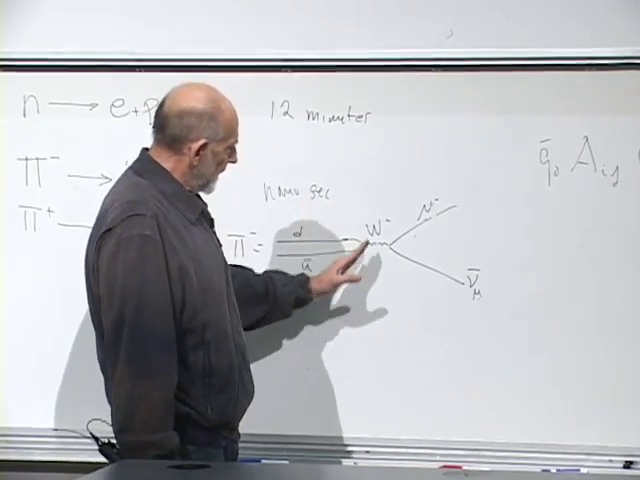
\includegraphics[width=0.72\textwidth]{lecture_05_figure_04.png}\caption{\(d\bar u\) 파이온이 가상 \(W^-\)로 소멸한 뒤 하전 렙톤과 이에 대응하는 반중성미자가 생성된다.}\lectureframe{01:19:38}\end{figure}

\begin{classroomqa}\audiencequestion{시간 방향을 세로가 아니라 가로로 그렸는데도 정말 파인만 다이어그램입니까?
\lecturetimestamp{01:20:21}}\lecturerresponse{그렇습니다. 페이지에서 시간을 어느 방향으로 나타낼지는 관례입니다. 한 방향을 시간으로 정하고 모든 화살표를 일관되게 해석하면, 그림은 동일한 상호작용 정보를 담습니다.}\end{classroomqa}

\begin{classroomqa}\audiencequestion{이 다이어그램을 비가역적인 일방향 붕괴라기보다 가역적인 화학 반응처럼 볼 수 있을까요?
\lecturetimestamp{01:21:35}}\lecturerresponse{역과정도 허용됩니다. 진공에서 생성된 파이온은 붕괴 생성물들이 서로 멀어져 보통은 다시 결합하지 않기 때문에 붕괴합니다. 하지만 뮤온과 반중성미자를 적절한 에너지와 운동량으로 함께 충돌시키면, 역상호작용을 통해 파이온을 형성할 진폭은 영이 아닙니다.}\end{classroomqa}

\subsection{에너지와 가상 중간 상태}

정지한 파이온에 대해,
\begin{equation}
m_\pi\simeq140\ {\rm MeV},
\qquad
m_\mu\simeq106\ {\rm MeV},
\qquad
m_\nu\approx0
\end{equation} 여기서 중요한 정밀도 수준에서는 이 정도다. 남은 에너지는 나가는 입자들의 운동 에너지가 된다. 운동량 보존에 따르면
\begin{equation}
\boldsymbol p_\mu+\boldsymbol p_{\bar\nu}=0,
\end{equation} 따라서 파이온 정지 좌표계에서 두 입자는 서로 반대 방향으로 날아간다.

\begin{classroomqa}\audiencequestion{\(W\)가 파이온보다 훨씬 무거운데 에너지가 어떻게 보존될 수 있습니까?
\lecturetimestamp{01:25:08}}\lecturerresponse{질량 껍질 위에 있어야 하는 것은 초기 입자와 최종 입자뿐입니다. 각 꼭짓점에서 사차원 운동량은 보존되지만 내부의 가상 선은 \(E^2=\boldsymbol p^2+m_W^2\)을 만족할 필요가 없습니다. 질량 껍질에서 벗어난 정도가 클수록 전파자가 과정을 더 강하게 억제합니다.\editorialnote{강의에서는 전통적인 에너지--시간 불확정성 표현을 사용하며 중간 상태가 짧은 시간 동안 에너지를 위반할 수 있다고 말한다. 더 정확한 현대적 설명은 답변에 제시된 것이다. 에너지와 운동량은 보존되지만 내부의 가상 선은 실제 입자의 질량 껍질 조건을 만족할 필요가 없다.}}\end{classroomqa}

\subsection{뮤온 붕괴}

뮤온은 먼저 가상 \(W^-\)를 방출하여 뮤온 중성미자로 바뀔 수 있다.
\begin{equation}
\mu^-\longrightarrow\nu_\mu+W^{-*}.
\end{equation} 이어서 가상 보손은 전자와 전자 반중성미자를 만든다.
\begin{equation}
\mu^-\longrightarrow
\nu_\mu+e^-+\bar\nu_e.
\label{eq:l5-muon-decay}
\end{equation} 이는 순수한 렙톤 과정이다. 뮤온은 전자보다 질량이 약 이백 배 크므로 최종 입자들의 정지 질량을 제하고도 운동 에너지로 쓸 에너지가 충분히 남는다.

\begin{figure}[htbp]\centering
\includegraphics[width=0.72\textwidth]{lecture_05_figure_06.png}\caption{가상 하전 약한 보손을 통한 뮤온 붕괴.}\lectureframe{01:29:24}\end{figure}

\begin{classroomqa}
\audiencequestion{전자와 함께 방출되는 중성 입자는 반중성미자인가요?
\lecturetimestamp{01:29:06}}
\lecturerresponse{그렇습니다. 완전한 최종 상태에는 뮤온 중성미자 하나, 전자 반중성미자 하나, 전자가 들어 있습니다. 맛을 나타내는 표지를 붙이면 두 중성 입자를 혼동하지 않을 수 있습니다.}
\end{classroomqa}

전자는 뮤온보다 가볍기 때문에 진공에서는 이 붕괴를 역으로 일으킬 수 없습니다. 타우는 더 무거워서 유사한 약한 상호작용 채널을 통해 붕괴할 수 있습니다. 여기서 안정성은 기초가 되는 꼭짓점의 차이 때문이 아니라, 부분적으로는 질량의 순서가 우연히 그렇게 정해져 있기 때문입니다.

\begin{classroomqa}
\audiencequestion{선형 가속기는 사실상 전자의 질량을 증가시켜, 그렇지 않으면 금지되는 반응을 반대 방향으로 일으키는 건가요?
\lecturetimestamp{01:30:23}}
\lecturerresponse{전자 고유 정지 질량을 바꾸지는 않지만 운동 에너지를 공급합니다. 충분한 질량중심 에너지가 있으면 더 무거운 최종 입자를 생성할 수 있으므로, 질량을 충돌에 이용 가능한 에너지로 바꾸어 말하면 제안하신 물리적 발상은 맞습니다.}
\end{classroomqa}

\subsection{쿼크 수준에서 본 중성자 베타 붕괴}

중성자와 양성자의 원자가 쿼크 조성은 다음과 같습니다.
\begin{equation}
n=udd,
\qquad
p=uud.
\end{equation}
중성자의 다운 쿼크 하나는 하전 전류 전이를 일으켜
\begin{equation}
d\longrightarrow u+W^{-*},
\end{equation}
\(udd\)에서 \(uud\)으로 바뀝니다. 이어서 가상 보손이 붕괴합니다.
\begin{equation}
W^{-*}\longrightarrow e^-+\bar\nu_e.
\end{equation}
두 꼭짓점을 결합하면 다음 과정이 재현됩니다.
\begin{equation}
n\longrightarrow p+e^-+\bar\nu_e.
\end{equation}

반대 방향의 쿼크 전이 \(u\to d+W^+\)가 일어나면 다운 쿼크 세 개로 이루어진 바리온이 생성되지만, 자유 중성자가 생성하기에는 그 상태의 질량이 너무 큽니다. 실제로 일어나는 다운에서 업으로의 전이는 에너지상 허용되는 경로입니다.

\begin{classroomqa}
\audiencequestion{중성자가 대신 양성자, 뮤온, 그리고 이에 대응하는 반중성미자로 붕괴할 수 있나요?
\lecturetimestamp{01:32:38}}
\lecturerresponse{정지해 있는 자유 중성자에서는 불가능합니다. 중성자--양성자 질량 차이는 뮤온 질량보다 훨씬 작습니다. 충돌이나 여기로 충분한 에너지를 더 공급하면, 같은 약한 상호작용 꼭짓점이 뮤온을 생성하는 채널에 관여할 수 있습니다. 금지되는 이유는 운동학적 제약이지, 상호작용이 없어서가 아닙니다.}
\end{classroomqa}

\section{아직 설명되지 않은 억제}

하전 약한 상호작용 꼭짓점으로 어떤 과정이 일어날 수 있는지는 설명되지만, 그 과정이 왜 그렇게 느린지는 아직 설명되지 않습니다. 약한 상호작용 결합이 유난히 작기 때문이라고 답하고 싶을 수도 있습니다. 그러나 그 답은 틀렸습니다. 무차원 약한 게이지 결합은 대략 전자기 결합과 비슷한 크기입니다. 억제의 원인은 다른 데서 찾아야 합니다.

빠진 요소는 가상 입자 전파자에서 이미 드러납니다. \(W\)은 매우 무겁습니다. \(m_W\)보다 훨씬 낮은 에너지에서는 하전 전류 진폭이 대략 \(1/m_W^2\)의 거듭제곱에 따라 억제됩니다. 힉스 메커니즘과 전약 대칭 깨짐을 통해 게이지 보손이 질량을 얻는 방식을 설명한 뒤 이 연결을 전개하겠습니다.
\editorialnote{이 강의에서는 이 문제를 다음 강의에서 다룰 수수께끼로 남겨 둡니다. 무거운 \(W\)에 대한 설명은 앞으로 이어질 내용을 미리 연결하기 위해 여기에 포함했으며, 이 강의에서 그 유도가 이루어졌다는 뜻은 아닙니다.}

\begin{classroomqa}
\audiencequestion{이 이론이 이러한 대칭성을 가진다고 할 때, 해당 변환에 대해 라그랑지안이 불변이라는 뜻인가요?
\lecturetimestamp{01:34:14}}
\lecturerresponse{맞습니다. 이론이 그 대칭성을 가진다는 말은 해당 변환에 대해 라그랑지안, 또는 동등하게 작용이 불변이라는 뜻을 줄여 표현한 것입니다. 라그랑지안 전체를 쓰는 일은 뒤로 미룬 것이지, 대칭성의 정의를 다른 것으로 바꾼 것이 아닙니다.}
\end{classroomqa}

이제 논의의 흐름이 완성되었습니다. 맥스웰 이론은 원형을 제시하고, 양자색역학은 비아벨 게이지 보손이 전하를 지니고 교환하는 방식을 보여 줍니다. 결합 상수는 원자 규모와 강입자 규모의 시간 척도 차이를 설명합니다. 그리고 약한 \(SU(2)\)은 쿼크와 렙톤을 \(W^\pm\)으로 묶어 줍니다. 이제 남은 과제는 기초 결합이 특별히 작지 않은데도 게이지 매개 과정이 실제로는 왜 약한지 이해하는 것입니다.